\setcounter{secnumdepth}{3}
\chapter{Requirements Engineering}
\label{sec:requirementsengineering}
Dieses Kapitel zeigt die speziellen Eigenschaften des Requirements Engineering im bereich der Webentwicklung.

Früh in der Entwicklung einer Software muss man die Rahmenbedingungen festlegen. Zuerst wird gezeigt, für welche Geräte und Browser man sich spezialisieren und generalisieren kann. 

Danach werden die wichtigsten nicht funktionalen Eigenschaften einer Webseite aufgezeigt und zum Schluss noch weitere wichtige Aspekte des Requirement Engineerings.

\section{Endgeräte}
Es gibt verschiedene Endgeräte, welche die Webseite darstellen müssen. 
\begin{itemize}
\item PC
\item Mobile
\item Tablet
\item E-Reader
\item Spielkonsolen
\end{itemize}

Als erster Punkt des Requirements Engineering sind die Geräte aufgeführt, da davon vieles abhängt. Zum Beispiel die Grösse des Bildschirmes, die Grösse des Eingabegerätes (Maus, Finger), die Bandbreite und noch weitere Punkte.

Für die verschiedenen Bildschirmgrössen gibt es zwei verschiedene Ansätze, die im Unterkapitel \ref{sec:requirementsengineerin:endgeraete:responsivevsadaptive} \nameref{sec:requirementsengineerin:endgeraete:responsivevsadaptive} beschrieben werden.

Dem Problem der Bandbreite nimmt sich das Kapitel \ref{sec:requirementsengineerin:endgeraete:bandbreite} \nameref{sec:requirementsengineerin:endgeraete:bandbreite} an.

\subsection{Responsive- vs Adaptive Web Design}
\label{sec:requirementsengineerin:endgeraete:responsivevsadaptive}
\footcite{Responsive_vs_Adaptive_Design_2015-05-31}
Beim \gls{rwdLabel} wird eine Seite generiert, die sich der Bildschirmgrösse anpasst, wo hingegen beim \gls{awdLabel} für verschiedene Bilschirmgrössen jeweils ein anderes Layout ausgeliefert wird.

\begin{figure}[H]
  \centering
  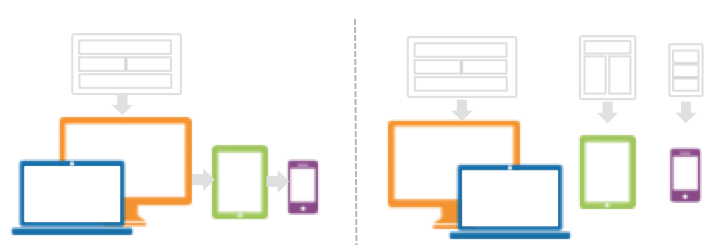
\includegraphics[width=0.9\textwidth]{images/rwd-vs-awd.png}
  \caption{Responsive- vs Adaptive Web Design\footcite{Responsive_vs_Adaptive_Design_for_UI_2015-05-31}}
  \label{fig:requirementsengineerin:endgeraete:responsivevsadaptive:comparision}
\end{figure}

Eim \gls{rwdLabel} liefert der Server für jedes Endgerät das selbe \Gls{glos:htmlLabel} aus. Die Elemente ordnen sich jedoch auf den verschiedenen Bildschirmgrössen anders an. Die folgende Grafik illustriert dieses vorgehen.

\begin{figure}[H]
  \centering
  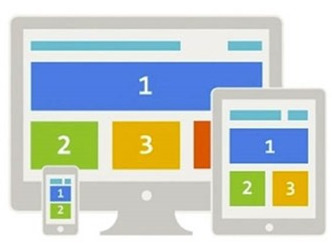
\includegraphics[width=0.4\textwidth]{images/rwd.jpg}
  \caption{Responsive Web Design\footcite{The_Difference_Between_Adaptive_Design_And_Responsive_Design_2015-05-31}}
  \label{fig:requirementsengineerin:endgeraete:responsivevsadaptive:rwd}
\end{figure}

Der Vorteil an dieser Variante ist es, dass keine Überprüfung der Bildschirmgrösse nötig ist und auf dem Bildschirm immer eine angepasste Ansicht ermöglicht wird. Auch wenn man die grösse des Browserfensters anpasst erhällt man immer eine passende Ansicht. Die Programmierung wird dadurch vereinfacht, dass nur eine \Gls{glos:htmlLabel} Seite generiert werden muss. Jedoch wird das Layout komplizierter und es müssen mehr Daten an das Engerät ausgeliefert werden.

Beim \gls{awdLabel} werden eigene \Gls{glos:htmlLabel} Seiten für die verschiedenen Auflösungen gepflegt. Um den selben Umfang wie das \gls{rwdLabel} zu ermöglichen, müssen die folgenden sechs Bildschirmbreiten gepflegt werden:
\begin{itemize}
\item 320px
\item 480px
\item 760px
\item 960px
\item 1200px
\item 1600px
\end{itemize}

Generell macht es Sinn ein \gls{rwdLabel} zu pflegen, da der Pflegeaufwand generell geringer ausfällt. Es gibt jedoch auch Gründe für ein \gls{awdLabel}. Zum Beispiel wenn eine bestehende Seite für mobile Geräte angepasst werden muss ist der Aufwand oft geringer, wenn man eine separate Ansicht dafür umsetzt. Die Ladezeiten für ein \gls{awdLabel} sind meistens auch besser, was folgende Tabelle aufzeigt. 
Für diesen Test\footcite{Adaptive_vs_Responsive_Web_Design_Which_Is_Right_for_Your_Site_-_Catchpoints_Blog_2015-06-01} wurden 15 Webseiten aus den \textit{Alexa Top 100 ranking (US)} Pages ausgesucht und analysiert.

\begin{center}
    \begin{tabular}{ | l | l | l |}
    \hline
    Metrik & \gls{awdLabel} & \gls{rwdLabel} \\ \hline
    Antwortzeit & 568 ms & 1'202 ms \\ \hline
    Zeit bis das Dokument vollständig geladen ist & 1'536ms & 4'086 ms \\ \hline
	Bytes Downloaded & 2'474'326 kB & 4'229'363 kB \\ \hline
	Objekte Downloaded & 20 & 61 \\ \hline
    \end{tabular}
\end{center}

Die \gls{awdLabel} Webseiten sind in allen Bereichen schneller. Es kann abschliessend gesagt werden, dass \gls{awdLabel} zu bevorzugen ist, wenn es auf die Geschwindigkeit ankommt. Dies war früher der Fall für mobile Endgeräte, fällt jedoch mit den neuen schnelleren Internetgeschwindigkeiten weniger ins Gewicht. Es sollte demnach wenn möglich \gls{rwdLabel} eingesetzt werden, ausser wenn die Migration einer bestehenden Webseite zu viel Aufwand bedeutet.


\subsection{Bandbreite}
\label{sec:requirementsengineerin:endgeraete:bandbreite}
Vor nicht all zu langer Zeit war die Bandbreite für Desktop PC's noch begrenzt und es musste sehr auf die Grösse von Bildern und Multimedia Inhalten geachtet werden. Doch das Internet entwickelte sich rasch weiter. Heute ist es möglich mehrere Full-HD (1980x1200 Pixel) Videos gleichzeitig anzusehen. Auf mobilen Endgeräten sieht es jedoch anders aus. Das \gls{wapLabel} wurde 1997 eingeführt. Auf grosse Grafiken musste man da noch verzichten da das Laden zu lange dauerte. Darauf folgte \gls{gprsLabel}, \gls{edgeLabel}, G3 und schlussendlich \gls{hsdpaLabel}. Mit den letzten beiden sind Webseiten und Bilder kein Problem mehr, und mit \gls{hsdpaLabel} können auch Multimedia Inhalte komfortable unterwegs angesehen werden. Die Abdeckung ist jedoch noch nicht flächendeckend. Vor allem in ländlichen Gebieten wird oft noch auf die älteren Verfahren zurückgegriffen. Deshalb muss für mobile Geräte die Bandbreite immer noch berücksichtigt werden.

Um die Bandbreite zu schonen werden Caches in den Browsern eingesetzt. Grosse Bilder, die auf mehreren Seiten vorkommen, zum Beispiel Banner, werden damit nur einmal heruntergeladen und auf dem Endgerät gespeichert. Dadurch ist nur der erste Seitenaufruf langsam. Die darauf folgenden Ladezeiten lassen sich jedoch beträchtlich vermindern.

\section{Browsers}
Jeder Webentwickler kennt die schmerzen, welche  die Entwicklung für verschiedene Browser mit sich bringt. Auch wenn das \gls{w3cLabel} vorgibt, wie eine \Gls{glos:htmlLabel} Dokument darzustellen ist, hat jeder Browser seine Eigenschaften auf welche Rücksicht genommen werden muss. Hier eine nicht abschliessende Liste von Browsern:
\begin{itemize}
\item Firefox
\item Chrome
\item Safari
\item Internet Explorer
\item Opera
\item Konqueror
\item Lynx
\end{itemize}
Es gibt verschiedene Versionen der Browser welche zusätzlich berücksichtigt werden muss und die meisten haben noch mobile Versionen.

Es ist wichtig, dass in den frühen Phasen eines Projektes festgelegt wird, welche Browser und Versionen unterstützt werden sollen, da dies einen grossen Einfluss auf den Aufwand hat.

\section{Nicht funktionale Eigenschaften}
\textit{Nicht funktionale Eigenschaften} sind solche, die nicht den Funktionsumfang der Software beschreiben. Von Kunden werden diese oft vergessen oder zu wenig Beachtung geschenkt. Noch für den Erfolg einer Webseite sind sie fast wichtiger als die eigentliche Funktionalität. Dies wurde eindrücklich mit der Einführung des IPhones gezeigt, denn dort stand die Geschwindigkeit und die Einfachheit der Benutzung im Vordergrund. Also zwei nicht funktionale Eigenschaften. 

Es gibt vier Eigenschaften für ein Projekt, die miteinander im Konflikt stehen:
\begin{itemize}
\item Zeit
\item Kosten
\item Funktionsumfang
\item Nicht funktionale Eigenschaften
\end{itemize}

Man muss sich entscheiden, auf welche Punkte besonders Wert gelegt werden. Denn alle vier Eigenschaften können nicht erreicht werden.

In diesem Kapitel werden folgende nicht funktionale Eigenschaften beschrieben:
\begin{itemize}
\item Geschwindigkeit
\item Sicherheit
\item Bedienbarkeit
\end{itemize}

\subsection{Geschwindigkeit}
Die Geschwindigkeit ist eines der wichtigsten Aspekte einer Seite. Es gibt diverse Statistiken welche aufzeigen, dass Benutzer die Webseite verlassen, wenn man zu lange warten muss. Es gibt drei Richtwerte\footcite{Response_Time_Limits_Article_by_Jakob_Nielsen_2015-06-01}.
\begin{itemize}
\item 0.1 Sekunden: Benutzer haben das Gefühl die Seite reagiert augenblicklich.
\item 1.0 Sekunden: Die Gedanken der Benutzer bleiben ununterbrochen.
\item 10 Sekunden: So lange wartet ein Benutzer ohne einer anderen Tätigkeit nachzugehen.
\end{itemize}
Wenn auf eine Aktion länger als eine Sekunde gewartet werden muss, soll muss dem Benutzer angezeigt werden, dass eine Aktion im Hintergrund durchgeführt wird. Dies kann durch einen sogenannten \textit{Spinner} visualisiert werden.

\begin{figure}[H]
	\begin{subfigure}{.3\textwidth}
	  \centering
	  
\includegraphics[width=.2\linewidth]{images/spinner1.jpeg}
	  \caption{Spinner 1}
	  \label{fig:requirementsengineerin:nichtfunktionale:geschwindigkeit:spinner:1}
	\end{subfigure}%
	\begin{subfigure}{.3\textwidth}
	 \centering
	 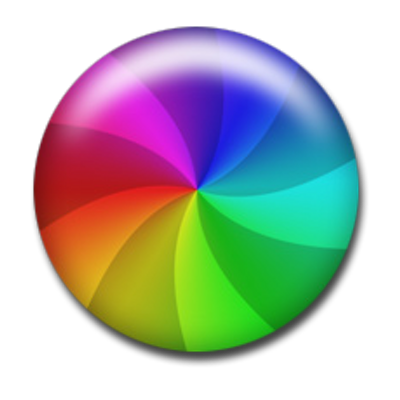
\includegraphics[width=.2\linewidth]{images/spinner2.png}
	 \caption{Spinner 2}
  	 \label{fig:requirementsengineerin:nichtfunktionale:geschwindigkeit:spinner:2}
	\end{subfigure}
	\begin{subfigure}{.3\textwidth}
	\centering
	
\includegraphics[width=.2\linewidth]{images/spinner3.png}
	\caption{Spinner 3}
 	 \label{fig:requirementsengineerin:nichtfunktionale:geschwindigkeit:spinner:2}
	\end{subfigure}
	\caption{plots of....}
	  \label{fig:requirementsengineerin:nichtfunktionale:geschwindigkeit:spinner}
\end{figure}

Schnelle Webseiten führen zu weniger Frustration, tieferen Blutdruck, tieferen Flow State und hören Umsatz\footcite{The_Psychology_of_Web_Performance_-_how_slow_response_times_affect_user_psychology_2015-06-01}.

Um die Geschwindigkeit zu verbessern kann Server- oder Client-Seitig Anpassungen vorgenommen werden. Je komplexer die Applikation ist, desto länger ist normalerweise auch die Ladezeiten. Es wurde gezeigt, dass durch eine Verkleinerung der Anzahl Zeilen an Sourcecode tendenziell auch die Ladezeiten vermindert werden\footcite{Web_Page_Performance_Thesis_-_web_page_response_time_measurement_modeling_and_monitoring_2015-06-01}.

\begin{figure}[H]
	\centering
	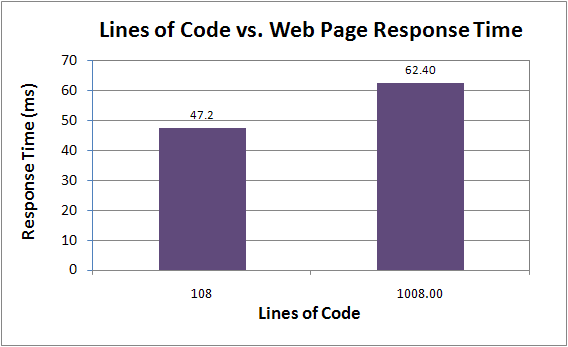
\includegraphics[width=.8\linewidth]{images/lines-of-code-response-time.png}
	\caption{Einfluss der Anzahl an Codezeilen auf die Ladezeit}
	\label{fig:requirementsengineerin:nichtfunktionale:geschwindigkeit:loc}
\end{figure}

Einen Einfluss auf die Ladezeit haben auch die Objekte welche von einer Seite geladen werden. Dies beinhaltet Bilder, \gls{cssLabel}- und \gls{jsLabel}-Files. Durch so genannte \textit{Sprite Sheets}. Das ist ein Bild, das mehrere Bilder enthält. Mittels \gls{cssLabel} kann das passende angezeigt werden. Hier ein beispielhaftes Sprite Sheet

\begin{figure}[H]
	\centering
	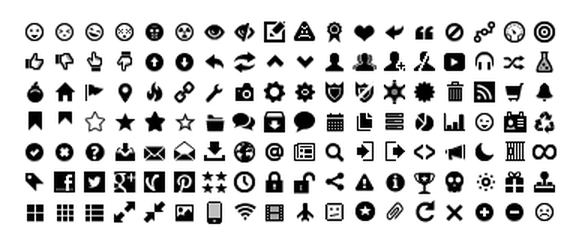
\includegraphics[width=.6\linewidth]{images/sprite_sheet.png}
	\caption{Sprite Sheet}
	\label{fig:requirementsengineerin:nichtfunktionale:geschwindigkeit:spritesheet}
\end{figure}

Auf der Client-Seite gibt es die Möglichkeit Objekte nachzuladen. Dadurch wird dem Benutzer rasch eine Seite dargestellt. Eine einfache Möglichkeit ist die Umstrukturierung der \Gls{glos:htmlLabel} Datei. \gls{cssLabel}- und \gls{jsLabel}-Dateien werden üblicherweise zu beginn definiert. Dadurch werden sie auch als erstes geladen wodurch es länger dauert bis dem User eine Webseite dargestellt wird. Wenn man die Referenz auf diese Files ans ende setzt, wird zuerst die Webseite geladen und dem Benutzer angezeigt. Dadurch wird die Reaktiontszeit kürzer.

Über \gls{ajaxLabel} kann über \gls{jsLabel} Code auf dem Client ausgeführt werden welcher Bilder, Dateien oder weiteren Code nachlädt. Bei dieser Variante ist jedoch zusätzliche Programmierung nötig und ist deshalb auch aufwändiger. 

\subsection{Sicherheit}
Beim Requirement Engineering sollte stets ein Entwickler, oder jemand der sich mit Sicherheit auskennt, anwesend sein. Denn dieses Thema wird sonst oft vergessen.

Die meisten Sicherheitslöcher bieten Formulare. Es kann über eine schlecht programmiertes Formular die gesamte Datenbank gelöscht oder ausgelesen werden, Spam-Emails versendet oder Schadcode eingespiesen werden.
Es wird hier nicht auf alle Sicherheitslöcher eingegangen. Exemplarisch wird hier die Ausnutzung von einer SQL-Injection gezeigt. Die folgende harmlose Adresse sollte nur etwas auslesen:

\begin{quote}
http://webserver/cgi-bin/find.cgi?ID=\textbf{42}
\end{quote}

Der generierte SQL-Code sieht folgendermassen aus:

\begin{quote}
SELECT author, subject, text FROM artikel WHERE ID=\textbf{42};
\end{quote}

Das Problem liegt darin, dass die 42 aus der Adresse direkt in die SQL Abfrage übernommen wird. Man könnte die Adresse nun folgendermassen verändern:

\begin{quote}
http://webserver/cgi-bin/find.cgi?ID=\textbf{42;UPDATE+USER+SET+\\
TYPE='admin'+WHERE+ID=23}
\end{quote}

Die neue SQL-Abfrage sieht nun so aus:


\begin{quote}
SELECT author, subject, text FROM artikel WHERE ID=\textbf{42;UPDATE USER SET TYPE='admin' WHERE ID=23}
\end{quote}

Es wird immer noch der Artikel mit der ID=42 ausgelesen, gleichzeitig gibt man dem eigenen Benutzer noch Administrator rechte.

Solche Fehler kann eine Firma viel Geld kosten und deren Ruf vernichten, weshalb die Sicherheit ein hoher Stellenwert in jeder Software bekommen sollte.

\subsection{Bedienbarkeit}
Wenn ein Benutzer eine Webseite bedienen bzw. navigieren kann ohne zu überlegen, so hat sie eine gute Bedienbarkeit. Doch dies umzusetzen ist nicht immer einfach. Die Navigation sowie der Aufbau der Seite müssen selbsterklärend sein. Dies muss schon wärend des Requirements Engineering geplant werden.

Bei grösseren Webseiten wird die Bedienbarkeit manchmal mittels \textit{Eye Tracking} überprüft. Dazu müssen Probanden ohne Vorkenntnisse vordefinierte Arbeitsschritte durchführen. Dabei wird aufgezeichnet, wo sie dabei auf der Webseite hinschauen. Dort wo am meisten hingesehen wird werden danach die wichtigsten Informationen platziert.

Alternativ können A/B-Tests durchgeführt werden. Möchte man zum Beispiel überprüfen, ob man mehr Produkte verkauft wenn die Navigation am oberen Bildschirmrand positioniert ist oder auf der linken Seite, so werden zwei Varianten programmiert. Variante A wird 50\% aller Webseitenbesucher angezeigt, Variante B den anderen 50\%. Dann wird gemessen, auf welcher Variante das bessere Resultat erzielt wird.

\section{Weiteres}
\subsection{Search Engine Optimisation}
Für einen erfolgreichen Webauftritt ist es essenziell, dass die Seite auf den diversen Suchmaschinen gefunden wird. Je weiter oben in der Suchresultate-Liste man erscheint desto besser. Dies ist das Ziel des  \gls{seoLabel}.

Suchmaschinen durchstöbern das Internet und untersuchen die Webseiten auf diverse Merkmale. Welche Merkmale ausgewertet und wie sie priorisiert werden ist ein gut gehütetes Geheimnis.

Wichtig ist sicherlich ein semantisch korrektes \Gls{glos:htmlLabel} Markup. Denn dadurch wird der Suchmaschine mitgeteilt, was eine Überschrift ist, was die wichtigsten Schlüsselwörter sind, welche anderen Seiten mit dieser in Beziehung stehen, etc. Dadurch kann der Inhalt von der Suchmaschine richtig ausgewertet werden.

Früher konnte man die Suchmaschinen überlisten, indem man die wichtigsten Schlüsselwörter oder Texte auf mehreren Seiten präsentierte. Diese wurden  als wichtig markiert. Heutige Suchmaschinen haben sich weiterentwickeln und erkennen jetzt so genannten \textit{duplicate content}. Ist duplicate content vorhanden wird dieser sogar als minderwertig markiert und das Suchresultat sinkt in der Suchresultat-Liste weiter herunter.

Die Suchmaschinen überprüfen auch, ob ein Text wirklich angezeigt wird. Ist ein Text nicht sichtbar für einen Benutzer, zum Beispiel durch weisse Schrift auf weissem Hintergrund, so wird der Inhalt auch nicht gewertet.

Auch die Position von Inhalten ist entscheidend. Je weiter oben etwas steht, desto wichtiger ist der Inhalt und desto weiter oben ist die Seite in der Suchresultat-Liste.

Es gibt Firmen welche sich nur auf \gls{seoLabel} spezialisiert haben. Dies zeigt die Wichtigkeit dieser Anforderung für den Erfolg einer Webseite. Der Aufwand sollte deshalb früh alloziert werden.

\subsection{Accessibility}
Der Grossteil Webseiten sind für "`normale"' Benutzer optimiert. Auch noch viele haben die Wichtigkeit von \gls{seoLabel} erkannt und ihre Webseiten dazu verbessert. Die Accessibility wird jedoch von fast keinen Webseiten umfassend implementiert. Dabei geht es darum, dass auch Benutzer mit eingeschränkten Möglichkeiten die Informationen von einer Webseite beziehen können. Damit sind hauptsächlich blinde Benutzer, also jene ohne einen Display gemeint.

Damit auch "`blinde"' Benutzer die Webseite voll umfänglich bedienen können müssen einige Punkte beachtet werden. Ein korrektes \Gls{glos:htmlLabel} Markup ist Voraussetzung. Dadurch wird dem User mitgeteilt, was ein Titel ist und was der Inhalt der Seite.

Bei Grafiken muss immer ein Bildbeschreibung angegeben werden. Dadurch weiss man, was das Bild darstellt, auch wenn man einen Browser besitzt der keine Bilder darstellen kann.

Für ältere Benutzer oder solche mit einer Sehschwäche ist es hilfreich, wenn man die Schriftgrösse anpassen kann. Es muss jedoch sichergestellt werden, dass dadurch das Layout der Seite nicht zerrissen wird.

Die meisten Webseiten haben keine speziellen Vorkehrungen getroffen für Benutzer mit einer Einschränkung. Das einzige was meistens vorhanden ist ist ein korrektes \Gls{glos:htmlLabel} Markup. Dieses wurde aber vielmehr für das \gls{seoLabel} gemacht als für die Accessibility.